\documentclass[openany, 12pt]{book}
\input{preamble}
\title{Github}
\author{Idris}
\date{August 2025}

% chktex-file 1
% chktex-file 2999999

\input{glossary}
\makeglossaries

\begin{document}

\tableofcontents

\part{CLI}

\part{API}

\begin{table}[h]
	\centering
	\rowcolors{2}{gray!10}{white}
	\begin{tabular}{ll}
		\toprule
		\textbf{Domain}        & \textbf{Description}                 \\
		\midrule
		Actions                & Workflow automation and CI/CD        \\
		Activity               & Events and notifications             \\
		Apps                   & GitHub Apps management               \\
		Billing                & Account and organization billing     \\
		Branches               & Branch management                    \\
		Campaigns              & Security and code scanning campaigns \\
		Checks                 & Status checks and results            \\
		Classroom              & GitHub Classroom integration         \\
		Code scanning          & Static analysis and results          \\
		Code security settings & Repo security configuration          \\
		Codes of conduct       & Repository CoC metadata              \\
		Codespaces             & Cloud development environments       \\
		Collaborators          & Repo collaborators and permissions   \\
		Commits                & Commit objects and history           \\
		Copilot                & GitHub Copilot APIs                  \\
		Credentials            & Credential management                \\
		Dependabot             & Dependency update automation         \\
		Dependency graph       & Dependency graph and insights        \\
		Deploy keys            & SSH deploy keys                      \\
		Deployments            & Deployment status and history        \\
		Emojis                 & Emoji metadata                       \\
		Gists                  & Gist objects and content             \\
		Git database           & Low-level Git objects                \\
		Gitignore              & Gitignore templates                  \\
		Interactions           & Interaction limits and moderation    \\
		Issues                 & Issue tracking                       \\
		Licenses               & License metadata                     \\
		Markdown               & Markdown rendering                   \\
		Meta                   & GitHub API metadata                  \\
		Metrics                & Usage metrics                        \\
		Migrations             & Repo/org migration                   \\
		Models                 & GitHub Models API                    \\
		Organizations          & Org management                       \\
		Packages               & GitHub Packages registry             \\
		Pages                  & GitHub Pages publishing              \\
		Private registries     & Private container/package registries \\
		Projects (classic)     & Project boards (classic)             \\
		Pull requests          & Pull request tracking                \\
		Rate limit             & API rate limit status                \\
		Reactions              & Reactions to issues/PRs/comments     \\
		Releases               & Release assets and metadata          \\
		Repositories           & Repo objects                         \\
		Search                 & Search across GitHub                 \\
		Secret scanning        & Secret scanning alerts               \\
		Security advisories    & Advisory publishing and management   \\
		Teams                  & Teams management                     \\
		Users                  & User objects and profiles            \\
		\bottomrule
	\end{tabular}
	\caption{GitHub API Domains}
\end{table}


\part{Actions}
\chapter{Workflow}

\begin{haskell}{}
-- a workflow is triggered by events and consists of jobs
data Workflow = Workflow
  { workflowName :: String
  , workflowOn   :: [Event]
  , workflowJobs :: [Job]
  }
\end{haskell}

\chapter{Event}
\begin{haskell}{}
-- triggering events
data Event =
      Push
    | PullRequest
    | Schedule String
    | ManualDispatch
\end{haskell}

\begin{table}[h]
	\centering
	\rowcolors{2}{gray!10}{white}
	\begin{tabular}{ll}
		\toprule
		\textbf{event}                & \textbf{trigger description}          \\
		\midrule
		\texttt{push}                 & any push to a branch or tag           \\
		\texttt{pull\_request}        & opened, synchronized, or closed pr    \\
		\texttt{workflow\_dispatch}   & manual trigger from ui or api         \\
		\texttt{repository\_dispatch} & external/custom trigger via api       \\
		\texttt{schedule}             & cron-like scheduled run               \\
		\texttt{release}              & published, edited, or deleted release \\
		\texttt{issue\_comment}       & comment added to an issue or pr       \\
		\texttt{issues}               & issue opened, edited, closed, etc.    \\
		\texttt{create}               & branch or tag created                 \\
		\texttt{delete}               & branch or tag deleted                 \\
		\texttt{fork}                 & repository forked                     \\
		\texttt{watch}                & user stars a repository               \\
		\texttt{workflow\_run}        & another workflow completes            \\
		\texttt{deployment}           & deployment event occurs               \\
		\texttt{deployment\_status}   & deployment status updates             \\
		\texttt{page\_build}          & github pages site is built            \\
		\texttt{package}              & package published or updated          \\
		\texttt{registry\_package}    & container/registry package activity   \\
		\texttt{discussion}           & discussion created, answered, etc.    \\
		\texttt{discussion\_comment}  & comment on a discussion               \\
		\texttt{check\_run}           & check run is created or completed     \\
		\texttt{check\_suite}         & check suite activity                  \\
		\bottomrule
	\end{tabular}
	\caption{Events that can trigger GitHub Actions workflows}
\end{table}

\chapter{Job}

\begin{haskell}{}
-- a job runs on a runner and is made up of steps
data Job = Job
  { jobName   :: String
  , jobRunsOn :: Runner
  , jobMatrix :: Maybe JobMatrix
  , jobSteps  :: [Step]
  }
\end{haskell}

\chapter{Job Matrix}
\begin{haskell}{}
-- matrix expansion for jobs
data JobMatrix = JobMatrix
  { matrixValues :: [(String, [String])]
  }
\end{haskell}

\chapter{Step / Action}
Actions are typically little more than wrappers around a single executable and
yet require substantial boilerplate to work properly. We can partition actions
into three buckets. The first are just git operations, like checkout, commit and
push.  The next is running programs, once they're installed of course, and then
getting some effect like API calls or filesystem changes. The last are actions
that call the github api, like updating releases, updating github pages, or
otherwise dealing with github stuff that is not just git.

\begin{table}[h]
	\centering
	\begin{tabular}{lll}
		\toprule
		\textbf{Group} & \textbf{Examples}                              & \textbf{Substrate}           \\
		\midrule
		Repo actions   & checkout, commit, push                         & Git repository / filesystem  \\
		program run    & nix build, etc, linters, compilers             & runner environment (cpu, fs) \\
		github api     & create release, label issue, merge pr, comment & github api / service state   \\
		\bottomrule
	\end{tabular}
	\caption{three categories of github actions}
\end{table}

\begin{table}[h]
	\centering
	\begin{tabular}{lll}
		\toprule
		\textbf{Action}                & \textbf{Purpose}          & \textbf{Typical Use Case}                  \\
		\midrule
		\multicolumn{3}{l}{\textbf{Repo actions}}                                                               \\
		\midrule
		\texttt{checkout}              & clone repo into runner    & make source available for build/test       \\
		\texttt{deploy-pages}          & publish to github pages   & deploy artifacts to pages branch           \\
		\texttt{download-artifact}     & retrieve stored outputs   & later jobs fetch artifacts for deploy/test \\
		\texttt{upload-artifact}       & store build outputs       & save pdfs, binaries, logs between jobs     \\
		\texttt{upload-pages-artifact} & stage site content        & prepare static site for pages              \\
		\midrule
		\multicolumn{3}{l}{\textbf{Runner setup / program run actions}}                                         \\
		\midrule
		\texttt{cache}                 & cache files between runs  & speed up builds (e.g.\ nix store)          \\
		\texttt{setup-node}            & install node.js           & js/ts builds or tooling                    \\
		\texttt{setup-python}          & install python            & python builds/tests or scripts             \\
		\texttt{setup-java}            & install jdk               & java/maven/gradle builds                   \\
		\texttt{setup-go}              & install go                & go project builds/tests                    \\
		\midrule
		\multicolumn{3}{l}{\textbf{GitHub API actions}}                                                         \\
		\midrule
		\texttt{create-release}        & create a release object   & publish tagged builds as releases          \\
		\texttt{labeler}               & auto-apply labels to PRs  & automate triage and categorization         \\
		\texttt{github-script}         & run JS against GitHub API & custom workflows beyond built-ins          \\
		\bottomrule
	\end{tabular}
	\caption{Core first-party GitHub Actions, partitioned by substrate}
\end{table}


\begin{haskell}{}
-- a step runs either shell commands or an action
data Step
  = Run String
  | Uses Action

-- reusable action
data Action = Action
  { actionName :: String
  , actionRepo :: String
  , actionRef  :: String
  }
\end{haskell}

\chapter{Runner}

\begin{figure}[H]
	\begin{center}
		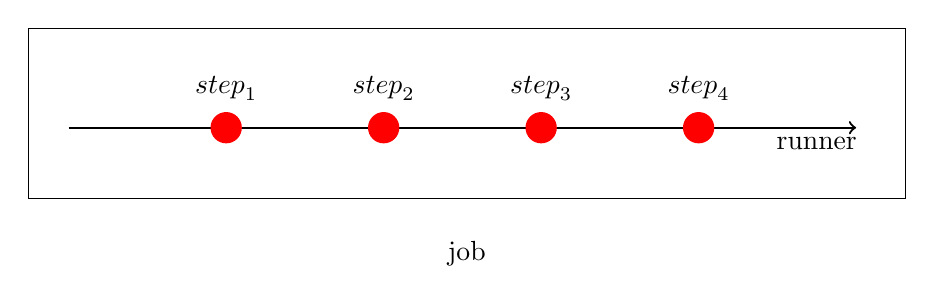
\begin{tikzpicture}
			\draw[thick, ->] (0,1) -- (10,1) node[pos=0.95, below] {runner}
			\foreach \p [count=\i from 1] in {0.2,0.4,0.6,0.8}
			{ node[pos=\p, circle, fill=red, inner sep=4pt, label=above:{$\text{step}_\i$}] {} };
			\draw[black]
			([xshift=-5mm,yshift=-5mm]current bounding box.south west)
			rectangle
			([xshift=5mm,yshift=5mm]current bounding box.north east)
			node[pos=0.5, below, yshift=-15mm] {job};
		\end{tikzpicture}
	\end{center}
	\caption{Runner with four steps}
\end{figure}

\begin{haskell}{}
-- runner types
data Runner
    = UbuntuLatest
    | WindowsLatest
    | MacOSLatest
    | SelfHosted [String] -- labels
deriving (Show, Eq)

-- extras
data Secrets   = Secrets   [(String, String)]
data Variables = Variables [(String, String)]
data Context   = Context    [(String, String)]

data Artifact  = Artifact
    { artifactName :: String,
      artifactPath :: FilePath }

data Cache     = Cache
    { cacheKey :: String,
      cachePath :: FilePath }
\end{haskell}

\chapter{Page}
Github pages is just some branch and directory combination which github then
statically serves under some github subdomain.

\begin{table}[h]
	\centering
	\begin{tabular}{lll}
		\toprule
		\textbf{Site Type} & \textbf{Branch}   & \textbf{Directory} \\
		\midrule
		Project Page       & \texttt{gh-pages} & \texttt{/} (root)  \\
		Project Page       & \texttt{main}     & \texttt{/docs}     \\
		Project Page       & \texttt{main}     & \texttt{/} (root)  \\
		User/Org Page      & \texttt{main}     & \texttt{/} (root)  \\
		\bottomrule
	\end{tabular}
	\caption{Valid GitHub Pages branch + directory combinations}
\end{table}

\chapter{App}
A github app is an external integration that authenticates to GitHub, subscribes
to webhooks, and calls the GitHub API.\@  It lives outside the Actions runtime, but
it can trigger workflows, comment on PRs, push commits, etc.

\end{document}
